%%%%%%%%%%%%%%%%%%%%%%%%%%%%%%%%%%%%
%% Template file SP 2024
%% Include in directory homework.sty and headerfooter.tex
%%%%%%%%%%%%%%%%%%%%%%%%%%%%%%%%%%%%

\documentclass[12pt]{article}
\usepackage{homework}

\graphicspath{{images/}}
\geometry{letterpaper, portrait, includeheadfoot=true, hmargin=1in, vmargin=1in}

\setcounter{section}{-1}
%% Solution hiding %%
\usepackage[utf8]{inputenc}
\usepackage{lipsum}


\begin{document}
\singlespacing

\renewcommand{\familydefault}{\rmdefault}
\pagestyle{fancy}
\fancyhf{}
\setlength{\headheight}{30pt}
\renewcommand{\headrulewidth}{0.4pt}
\renewcommand{\footrulewidth}{0.4pt}
\lhead{\large Homework 2 \\ Due Feb. 20, 2024 }
\rhead{\large CS 446 \\ Spring 2024}
\rfoot{\textbf{Page \thepage}}
\lfoot{}

\section{Instructions}

Homework is due Tuesday, February 20, 2024 at 23:59pm Central Time.
Please refer to \url{https://courses.grainger.illinois.edu/cs446/sp2024/homework/hw/index.html} for course policy on homeworks and submission instructions.

\section{Soft-margin SVM: 4pts}
The Lagrangian form of the soft-margin SVM is given by
\begin{eqnarray}
    L(\omega, b, \xi, \alpha, \beta) &=& \frac{1}{2}||\omega||^2 + C\sum_{i=1}^n \xi_i - \sum_{i=1}^n \alpha_i[y_i(\omega^Tx_i + b) - 1 + \xi_i] - \sum_{i=1}^n \beta_i\xi_i \nonumber
\end{eqnarray}
The dual form of the problem is then given by
\begin{eqnarray}
    D(\alpha, \beta) = \min_{\omega, b, \xi} L(\omega, b, \xi, \alpha, \beta) \nonumber
\end{eqnarray}
Because the problem is convex, we know that the maximum of the dual is the minimum of the primal. The solution to the dual occurs when the gradients of the Lagrangian are 0, i.e.
\begin{eqnarray}
    \nabla_{\omega}L(\omega, b, \xi, \alpha, \beta) &=& \omega - \sum_{i=1}^n \alpha_iy_ix_i = 0 \nonumber \\
    \nabla_{b}L(\omega, b, \xi, \alpha, \beta) &=& -\sum_{i=1}^n \alpha_iy_i = 0 \nonumber \\
    \nabla_{\xi}L(\omega, b, \xi, \alpha, \beta) &=& C - \alpha_i - \beta_i = 0 \nonumber
\end{eqnarray}
Substitue these back into the Lagrangian, we have
\begin{eqnarray}
    D(\alpha, \beta) &=& \frac{1}{2}||\sum_{i=1}^n \alpha_iy_ix_i||^2 + C\sum_{i=1}^n \xi_i - \sum_{i=1}^n \alpha_i[y_i(\sum_{j=1}^n \alpha_jy_jx_j^Tx_i + b) - 1 + \xi_i] - \sum_{i=1}^n \beta_i\xi_i \nonumber
    \\ &=& \sum_{i=1}^n \alpha_i - \frac{1}{2}\sum_{i=1}^n\sum_{j=1}^n\alpha_i\alpha_jy_iy_jx_i^Tx_j \nonumber 
\end{eqnarray}
subject to
\begin{eqnarray}
    \alpha_i &\geq& 0 \nonumber \\
    \beta_i &\geq& 0 \nonumber \\
    \alpha_i + \beta_i &=& C \nonumber \\
    \sum_{i=1}^n \alpha_iy_i &=& 0 \nonumber
\end{eqnarray}

After eliminating $\beta_i$, we have the following constraints,
\begin{eqnarray}
    0 \leq \alpha_i &\leq& C \nonumber \\
    \sum_{i=1}^n \alpha_iy_i &=& 0 \nonumber
\end{eqnarray}

\newpage

\section{SVM, RBF Kernel and Nearest Neighbor: 6pts}
\subsection{}
\begin{eqnarray}
    \hat{\omega} &=& \sum_{i=1}^N \hat{\alpha}_iy_ix_i \nonumber\\
    f(x) &=& (\sum_{i=1}^N \hat{\alpha}_iy_ix_i)^T x \nonumber
\end{eqnarray}

\subsection{}
\begin{eqnarray}
    \hat{\omega} &=& \sum_{i=1}^N \hat{\alpha}_iy_i\phi(x_i) \nonumber \\
    f(x) &=& (\sum_{i=1}^N \hat{\alpha}_iy_i\phi(x_i))^T \phi(x) \nonumber \\ 
        &=& \sum_{i=1}^N \hat{\alpha}_iy_iK(x_i, x) \nonumber
\end{eqnarray}

\subsection{}
\begin{eqnarray}
    \lim_{\delta \to 0} \frac{\sum_{i=1}^{N}{\hat{\alpha}y_ie^{-\frac{||x_i-x||^{2}}{2\delta^{2}}}}}{e^{-\frac{\rho ^2}{2\delta^{2}}}}
    &=& \lim_{\delta \to 0} \sum_{i=1}^{S}{\hat{\alpha}y_ie^{-\frac{||x_i-x||^{2} - \rho ^2}{2\delta^{2}}}} \nonumber \\
    &=& \lim_{\delta \to 0} \sum_{i=1}^{T}{\hat{\alpha}y_ie^{-\frac{||x_i - x||^{2} - \rho^2}{2\delta^2}}} 
    +  \lim_{\delta \to 0} \sum_{i=1}^{S/T}{\hat{\alpha}y_ie^{-\frac{||x_i - x||^{2} - \rho^2}{2\delta^2}}} \nonumber \\
    &=& \sum_{i=1}^{T}{\hat{\alpha}y_i + 0} \nonumber 
\end{eqnarray}

\newpage

\section{Decision Tree and Adaboost: 12 pts}
\subsection{}
From the definition of entropy, we have
\begin{eqnarray}
    I(D) &=& -\sum_{c=1}^C p(c|D)\log_2p(c|D) \nonumber \\
    &=& -\frac{1}{2}\log_2\frac{1}{2} - \frac{1}{2}\log_2\frac{1}{2} \nonumber \\
    &=& 1 \nonumber
\end{eqnarray}

\subsection{}
First consider split on $x_1$. Split points between two adjacent points can be considered as same, so we have possible split points at $\tau = 2, 3, 4, 5, 6$. 
For each $\tau$, we split the dataset following the rule $y = 1$ if $x \ge \tau$, otherwise $y = -1$.
\begin{eqnarray}
    I(D|f_{\tau=2}) = 0.809, I(D|f_{\tau=3}) = 1, I(D|f_{\tau=4}) = 0.918, I(D|f_{\tau=5}) = 0.541, I(D|f_{\tau=6}) = 0.809 \nonumber
\end{eqnarray}
So the best split for $x_1$ is at $\tau = 5$.

Similarly, we have possible split points at $\tau = 2, 3, 4, 5, 6$ for $x_2$, following the rule $y = -1$ if $x \ge \tau$, otherwise $y = 1$.
\begin{eqnarray}
    I(D|f_{\tau=2}) = 0.809, I(D|f_{\tau=3}) = 1, I(D|f_{\tau=4}) = 0.918, I(D|f_{\tau=5}) = 1, I(D|f_{\tau=6}) = 0.809 \nonumber
\end{eqnarray}
So the best split for $x_2$ is at $\tau = 2$ and $\tau = 6$. Since the information gain split on $x_1$ is higher, we choose to split on $x_1$ at $\tau = 5$.
\begin{eqnarray}
    IG(D, f) = I(D) - I(D|f) = 0.459 \nonumber
\end{eqnarray}

\subsection{}
After split on $\tau = 5$, from the figure we can know that only split on $x_2$ at $\tau = 2$ can further reduce the entropy. So the best split for the second level is at $\tau = 2$, following the rule $y = -1$ if $x \ge \tau$, otherwise $y = 1$.
\begin{eqnarray}
    I(D|f_{x_1=5, x_2=2}) &=& \frac{1}{6}0 + \frac{1}{2}0 + \frac{1}{3}0 = 0 \nonumber\\
    IG(D|f_{x_1=5}, f_{x_2=2}) &=& I(D|f_{x_1=5}) - I(D|f_{x_1=5, x_2=2}) = 0.541 \nonumber 
\end{eqnarray}
So, after the second split, the further information gain is 0.541. The total information gain is $ 0.459 + 0.541 = 1$.

\subsection{}
Follow the Adaboost routine, at $t = 1$, we have,
\begin{eqnarray}
    \gamma_1^{i} &=& \frac{1}{6} \nonumber \\
    f_1(x) &=& \begin{cases}
        1, & x_1 \ge 5 \\
        -1, & x_1 < 5
        \end{cases} \nonumber \\
    z_1 &=& \sum_{i = 1}^{6} \frac{1}{6} y^{i} f_1(x_i) = \frac{4}{6} \nonumber \\
    \alpha_1 &=& \frac{1}{2}\ln\frac{1 + z_1}{1 - z_1} = \frac{1}{2}\ln 5 \nonumber \\
    \gamma_2^2 &=& \frac{1}{6 Z _1}e^{-\frac{1}{2}\ln 5 (-1)} \nonumber \\
    \gamma_2^i &=& \frac{1}{6 Z _1}e^{-\frac{1}{2}\ln 5 }, i \ne 2 \nonumber 
\end{eqnarray}
After the normalization, we have $\gamma_2^2 = \frac{1}{2}$, $\gamma_2^i = \frac{1}{10}, i \ne 2$. Thus, at $t = 2$, we have,
\begin{eqnarray}
    f_2(x) &=& \begin{cases}
        -1, & x_2 \ge 4 \\
        1, & x_2 < 4
        \end{cases} \nonumber \\
    z_2 &=& \sum_{i = 1}^{6} \gamma_2^i y^{i} f_2(x_i) = \frac{3}{5} \nonumber \\
    \alpha_2 &=& \frac{1}{2}\ln\frac{1 + z_2}{1 - z_2} = 0.6931 \nonumber 
\end{eqnarray}

\subsection{}
The final classifier is given by
\begin{eqnarray}
    f(x) = sign(0.8047 * f_1(x) + 0.6931 * f_2(x)) \nonumber \\
    where \quad f_1(x) &=& \begin{cases}
        1, & x_1 \ge 5 \\
        -1, & x_1 < 5
        \end{cases} \nonumber \\
    f_2(x) &=& \begin{cases}
        -1, & x_2 \ge 4 \\
        1, & x_2 < 4
        \end{cases} \nonumber
\end{eqnarray}
\begin{eqnarray}
    f(x_1) &=& sign(0.8047*(-1) + 0.6931*(1)) = -1 \quad \text{correct}\nonumber \\
    f(x_2) &=& sign(0.8047*(-1) + 0.6931*(1)) = -1 \quad \text{incorrect} \nonumber \\
    f(x_3) &=& sign(0.8047*(-1) + 0.6931*(-1)) = -1 \quad \text{correct} \nonumber \\
    f(x_4) &=& sign(0.8047*(-1) + 0.6931*(-1)) = -1 \quad \text{correct} \nonumber \\
    f(x_5) &=& sign(0.8047*(1) + 0.6931*(1)) = 1 \quad \text{correct} \nonumber \\
    f(x_6) &=& sign(0.8047*(1) + 0.6931*(-1)) = 1 \quad \text{correct} \nonumber
\end{eqnarray}

\newpage

\section{Learning Theory: 14pts}
\subsection{}
From Hoeffding's inequality, with probability at least $0.95$, we have
\begin{eqnarray}
    \epsilon_{\mu}(h) &\le& \epsilon_{\mathcal{D}}(h) + \sqrt{\frac{\log(\frac{2}{\delta})}{2n}} \nonumber
\end{eqnarray}
Since, we want to have $\epsilon_{\mu}(h) - \epsilon_{\mathcal{D}}(h) \le 0.05$, we have,
\begin{eqnarray}
    \sqrt{\frac{\log(\frac{2}{\delta})}{2n}} &\le& 0.05 \nonumber \\
    n &\ge& 200 \log 40 \nonumber \\
    n &\ge& 738 \nonumber
\end{eqnarray}

\subsection{}
\subsubsection{}
$\mathsf{V} \mathsf{C} (\mathcal{F} _{\text{affine}}) = 3$.

We can image this function as a line in 2D space, and the objective is to seperate the points into two classes. Points above the line are labeled as 1, and points below the line are labeled as -1. For 3 points not in the same line, we can always find a line to seperate them. 

On the other hand, for any dataset containing 4 points, if there are 3 points in a line, they cannot be seperated. Otherwise, there are at least 4 points forming in a XOR pattern so that we cannot seperate as well. So the VC dimension of $\mathcal{F} _{affine}$ is 3.

\subsubsection{}
$\mathsf{V} \mathsf{C} (\mathcal{F}^{k} _{\text{affine}}) = k+1$.

Rewrite the definition of $\mathcal{F}^{k} _{\text{affine}}$ as $\mathcal{F}^{k} _{\text{affine}} = \{ \mathbb{I} \{ \left [ x^T \quad 1 \right ]  \begin{bmatrix} \mathbf{\omega}\\\omega_0 \end{bmatrix}  \}\}$.
The first matrix $\mathbf{X} $ is of $\mathbb{R} ^{n\times( k+1 ) }$, the second matrix $\mathbf{W} $ is of $\mathbb{R} ^{(k+1)\times 1}$. 
For $n=k+1$, we know that the first matrix is of full rank, so we can always get a solution to the problem $\mathbf{X} \mathsf{W} = \mathbf{Y} $, where $\mathbf{Y} $ is arbitrary labels for points.

On the other hand, for $n = k+2$, i.e. there are $k+2$ points in $\mathbb{R}^{k+1}$ space, thus there exists a point $x_j = \sum_{i\ne j} a_{i}x_{i}$, where not all $a_{i}$ are $0$. Assign label for $x_j$ as 1 and $sign(a_i)$ for other $y_i$s, we know that $y_{i} = sign(a_{i})$ is achieved by $sign (W^T x_{i})$. If $a_i = 0$, the label is arbitrary.
Then we have $sign(w^Tx_{j}) = sign(\sum_{i \ne j}a_{i}w^Tx_{i})$. The signs of $w^Tx_{i}$ is the same as $a_{i}$, thus we get $sign(w^Tx_{j}) = y_{j} > 0$, which is Contradictory to our assumption. So we know that the VC dimension of $\mathcal{F}^{k} _{\text{affine}}$ is $k+1$.

\subsubsection{}
$\mathsf{V} \mathsf{C} (\mathcal{F}^{k} _{\text{cos}}) = infinite$. 


\section{Coding: SVM, 4pts}
% Include your plot for Q5.3.
\begin{figure}[h]
    \centering
    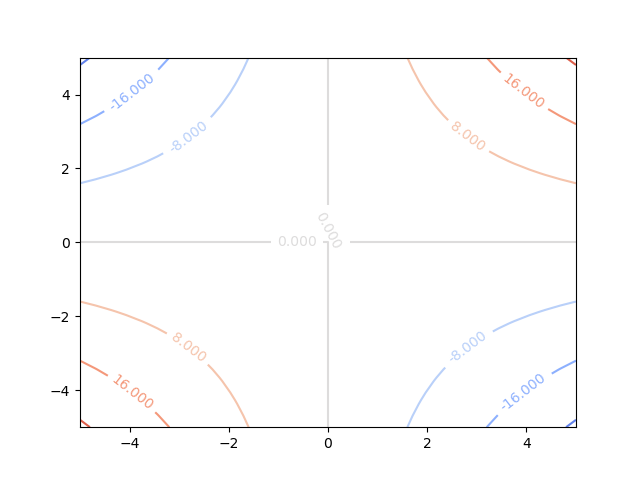
\includegraphics[width=0.5\textwidth]{imgs/poly_2.png}
    \caption{Results of Polynomial kernel degree of 2}
    \end{figure}

    \begin{figure}[h]
        \centering
        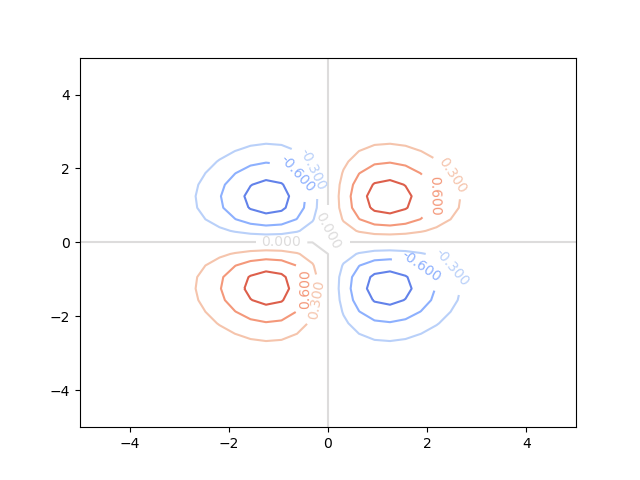
\includegraphics[width=0.5\textwidth]{imgs/rbf_1.png}
        \caption{Results of RBF kernel with $\gamma = 1$}
    \end{figure}
    
    \begin{figure}[h]
        \centering
        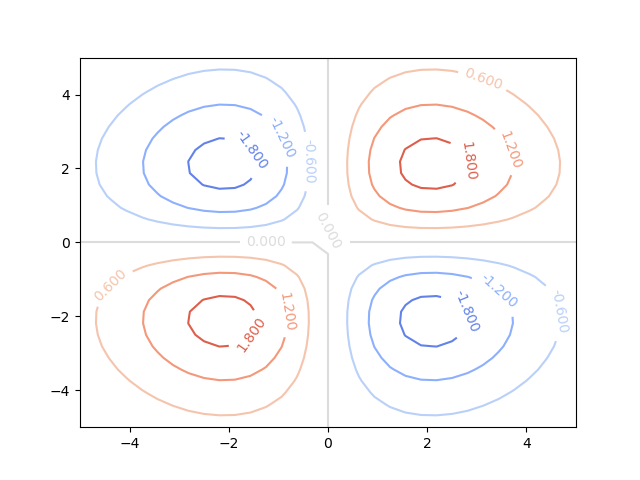
\includegraphics[width=0.5\textwidth]{imgs/rbf_2.png}
        \caption{Results of RBF kernel with $\gamma = 2$}
    \end{figure}

    \begin{figure}[h]
        \centering
        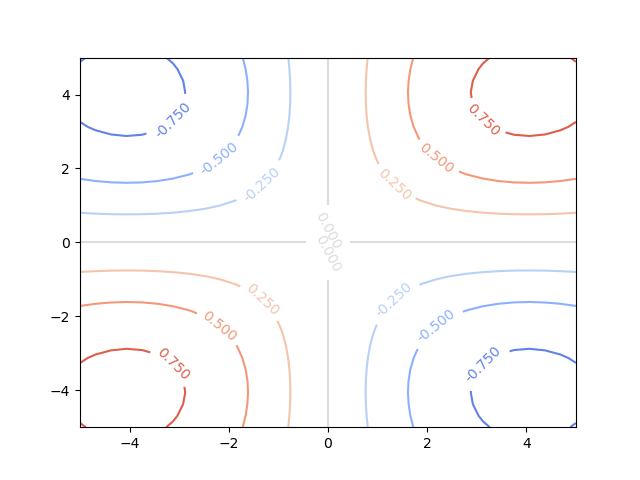
\includegraphics[width=0.5\textwidth]{imgs/rbf_4.png}
        \caption{Results of RBF kernel with $\gamma = 4$}
    \end{figure}
    
\end{document}